% En este capitulo se presentan y analizan los resultados experimentales de la
% solucion para el problema de al exploración multi-robot coordinada que fue
% desarrollada en este proyecto.

% Las pruebas realizadas se separan en tres secciones según su proposito. La
% primera estudia el impacto de construir el GVD de forma incremental. La
% segunda compara las diversas tecnicas de identificación de objetivos. Y la
% tercera analiza la influencia de las diversas formas de considerar el espacio
% desconocido. 


% Las pruebas realizadas tienen  propositos,  para estudiar el impacto de
% construir el GVD de forma incremental. Para comparar las diversas tecnicas de
% identificación de objetivos. Y finalmente para analizar la influencia de las
% diversas formas de considerar el espacio desconocido. 

% , se presentan los resultados obtenidos y analizan
%  los resultados los cuales son analizados.

% Comentar que estos son cosas generales a todas las pruebas, que en cada una de
% las siguientes secciones se cambian paramtros aislados con el proposito de
% comparar su impacto. (ver capaz que crierios se van a comparar en cada una)

% generales de las pruebas realizadas. Estas 

Este capitulo está dedicado a describir las pruebas realizadas y analizar sus 
resultados. Las pruebas se llevaron a cabo en un simulador y consisten
en resolver una instancia del problema de exploración multi-robot
con distintas soluciones.
Los resultados de las pruebas se presentan y analizan en cuatro secciones. En
la sección \ref{sec:exp:cubcal} se evalúan los mapas construidos en las
pruebas. En la sección \ref{sec:exp:inc} se estudia el impacto de construir el
GVD de forma incremental. En la sección \ref{sec:exp:idobj} se comparan las
diversas técnicas de identificación de objetivos. Y finalmente, en la sección
\ref{sec:exp:desco} se analiza el efecto de considerar el
espacio desconocido de distintas formas. 



\section{Especificación de las pruebas}

A lo largo de esta se sección se especifican las pruebas realizadas en este proyecto.
 % y presentadas a lo largo de este capitulo.
% * Pruebas realizadas, cosas generales:
%   * simulador
%   * hardware (de mi pc)
%   * Los robots utilizados
%     * sensor 
%     * robot en si
%   * El entorno de pruebas
%   * Criterios utilizados para analizar los resultados: 
%     * Referencias
%     * Explicar cuales son
%   * Cantidad de pruebas, promedio y varianza

% cuyos resultados se
% presentan a lo largo del capitulo.

% En esta seccion se plantean las caracteristicas generales que comparten todas
% las pruebas que se presentan a lo largo del capitulo.

% En lo que resta de esta seccion se especifican las caracteristicas de las
% pruebas llavadas a cabo. 

% A lo largo del capitulo se presentan diversas pruebas que buscan comparar ciertos
% aspectos de la solucion desarrollada en este proyecto. En esta seccion se
% especifican las caracteristicas generales que comparten todas las pruebas
% realizadas.

% En esta sección se establecen als car


% \subsection{Tipos de prueba}
% El proposito de las pruebas presentadas es evaluar el desempeño de diversos aspectos de una
% solucion al problema de la exploción multi-robot. 
% Los tipos de prueba quedan definidos 

% Las pruebas tienen como proposito validar las variantes presentadas para la
% solucion de diviersos aspectos de la del problema de exploración multi-robot.
 
% Para lograr esto se definen pruebas consisten en reslover una instancia de
% dicho problema, cambiando la forma de resolver cada aspecto a validar.

% La instancia del problema de exploración a resolver es el de explorar un
% entorno cerrado con una flota de robots, hasta que no exista espacio sin
% explorar.

% Debido a esto
% las pruebas se dividen en tres secciones, dependiendo del aspecto que se busca comparar.
% Dado esto las pruebas

% En la seccion \ref{sec:exp:inc} se compara la construccion incremental del GVD contra
% la no incremental, en la seccion \ref{sec:exp:idobj} se
% comparan los metodos de identificación de objetivos que se describen en la seccion
% \ref{sec:pc:idobj}, finalmente en la seccion 
%  la seccion \ref{sec:exp:desco} analiza la
% influencia de las diversas formas de considerar el espacio desconocido. 

% de objetivos que
% utiliza directamente las fronteras como objetivos, con las que se basan en
% simplicar dichas fronteras, tanto la simplificación basada en K-Means, como la
% basada en cubrimiento. 

% Dado que se quiere comparar la utilidad entre las variantes para ciertas partes de
% la solución, se definen tipos de prueba según las variantes utilizadas. 
% En esta sección se describe el tipo de prueba que se denominara como $base$. Este consiste
% en una solucion del problema de exploración multi-robot que 
 % La solución base consiste en resolver la
% asignación de objetivos basada en cubrimiento (seccion \ref{subsec:MiSimp}). La as La construccion de GVD
% incremental como es comentada en \ref{sec:MiConstGVD} con

\subsection{Simulador}
Las pruebas fueron simuladas con Gazebo \cite{gazebo}, el cual fue elegido a
partir del análisis comparativo entre varios simuladores candidatos realizado
en la sección \ref{sec:sim}. 

\subsection{Tipos de pruebas}
Las pruebas consisten en resolver una instancia del problema de exploración
multi-robot. Específicamente en explorar un entorno cerrado con una flota de
robots hasta no detectar más espacio desconocido explorable. 

El propósito de las pruebas es evaluar ciertos aspectos de la solución
propuesta en este proyecto para dicho problema. Para lograr evaluar cada
aspecto por separado se ejecutan pruebas tanto con la solución como fue
propuesta originalmente, como con variantes de la misma que cambian únicamente
el aspecto a evaluar. Los aspectos de la solución original a evaluar son: la construcción incremental
del GVD (sección \ref{sec:MiConstGVD}). La identificación de objetivos que
simplifica las fronteras basándose en el cubrimiento (sección
\ref{subsec:MiSimp}). Y la consideración del espacio desconocido al construir
el GVD presentada en la sección \ref{subsec:espDesc}, donde las celdas
desconocidas no propagan ondas y el conjunto $\mli{UF}$ de celdas desconocidas
que son adyacentes a celdas libres pertenecen a generadores ($\mli{UF}
\subseteq \mli{CGen}$).


 % permite evaluar el desempeño de
% una solución que resuelve dicho problema. El caso de pruebas definido
% El tipo de mapa
% generado en la exploración es una grilla de ocupación de un tamaño fijo
% suficiente para representar el entorno explorado.
% Para validar la construccion incremental del GVD esta se compara contra la
% construccion no incremental. En el caso de la identificación de objetivos se
% comparan las tres estrategias propuestas en la seccion \ref{sec:pc:idobj}: el
% identificar las fronteras como objetivos, simplicar dichas fronteras a partir
% K-Means, y simplificarlas basandose en el cubrimiento. Por último, la
% consideracion del espacio desconocido en la contruiccion del GVD se valida
% comparandola contra considerar que el espacio desconocido es libre. 

Para evaluar la construcción incremental del GVD se compara contra el método de 
construcción no incremental brushfire (sección \ref{subsec:constGVD}). En el caso de la
identificación de objetivos se compara contra identificar todas las fronteras
como objetivos (sección \ref{subsec:todasFront}), y la técnica que identifica
objetivos simplificando dichas fronteras a partir K-Means (sección
\ref{subsec:simpKM}). Por último, la consideración del espacio desconocido en
la construcción del GVD se compara contra considerar que el espacio
desconocido es libre (sección \ref{subsec:espDesc}). 

Se prueban entonces cinco soluciones, la que utiliza todos los aspectos a
evaluar a la vez y las restantes cuatro que difieren de la primera únicamente
en uno de dichos aspectos.

Con el motivo de probar distintas cargas computacionales, cada prueba se repite
cambiando la granularidad de la grilla de ocupación utilizada para representar
el entorno explorado. La granularidad se indica a través de la cantidad de
celdas de la grilla que corresponden a un metro cuadrado de la realidad. Los
valores de granularidad utilizados para las pruebas son $1,4,9$ y $16$ celdas
por metro cuadrado ($\frac{celdas}{m^2}$). 

Adicionalmente debido a que es posible que ejecuciones de un misma simulación
lleven a distintos resultados, con el fin de obtener resultados
estadísticamente significativos cada prueba fue ejecutada 20 veces. Siendo 
$5*4*20=400$ el total de pruebas ejecutadas.
% las tres tecnicas, identfica todas las fornteras como objetivos, 

% Debido a esto
% las pruebas se dividen en tres secciones, dependiendo del aspecto que se busca comparar.
% Dado esto las pruebas

% Para cumplir con la hipotesis (IV) planteada en \ref{sec:hip}
\subsection{Entorno}
Las pruebas se realizan en un entorno cerrado que tiene un área explorable de
aproximadamente $10000m^2$. El entorno está estructurado en habitaciones,
puertas y corredores de varios tamaños. Los únicos obstáculos presentes en él
son paredes y los mismos robots que pueden obstaculizarse entre
sí. Un mapa de este entorno se muestra en la figura
\ref{fig:willow}.

\begin{figure}[H]
  \center
  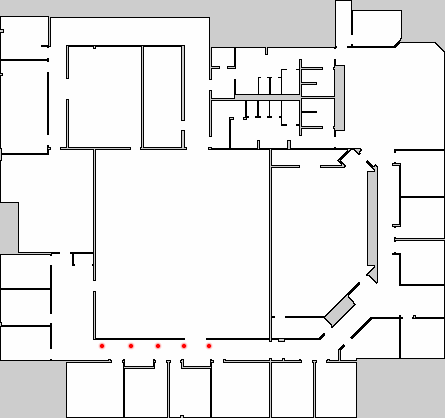
\includegraphics[width=0.5\linewidth]{imagenes/willow/0_250000mRobots2.png}
  \caption[Mapa del entorno utilizado en las pruebas.]{Mapa del entorno utilizado en las pruebas. En negro se indican las paredes, en blanco el espacio libre y en gris el espacio inaccesible. Las posiciones iniciales de los robots se indican en rojo.}
  \label{fig:willow}
\end{figure} 

El entorno fue construido a partir de un modelo que se encuentra disponible por
defecto en Gazebo, llamado \say{Willow Garage}, el cual se modifico para
reducir el área a explorar y que sea cerrado (sin salidas al exterior).

\subsection{Robots}
Los robots simulados\footnote{Especificación disponible en línea:\\
\url{https://gitlab.fing.edu.uy/federico.ciuffardi/pioneer_p3dx_model}.\\ Accedido por última vez: 25/02/2022.} utilizados en las
pruebas modelan al robot diferencial Pioneer 3-DX \cite{p3dx} (figura
\ref{fig:p3dx}). Cada robot está equipado con un sensor \gls{LiDAR} basado en el
modelo URG-04LX-UG01 \cite{hokuyo}, que permite tomar medidas de distancia de
hasta $5.6m$, con una frecuencia de $10hz$ de un máximo de $36hz$.
Adicionalmente el sensor fue alterado para tomar medidas en los $360$\textdegree
al rededor del robot y para proporcionar medidas perfectas (sin ruido).

\begin{figure}[H]
  \centerfloat

  \subfloat[Real.]{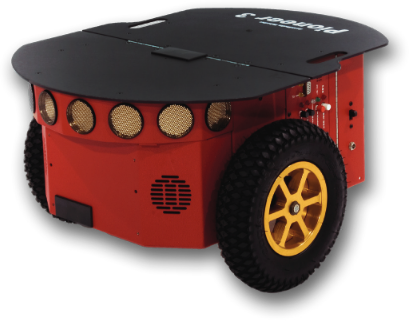
\includegraphics[clip=true, width=0.33\textwidth]{imagenes/pion/real.png}}
  \qquad
  \subfloat[Simulado.]{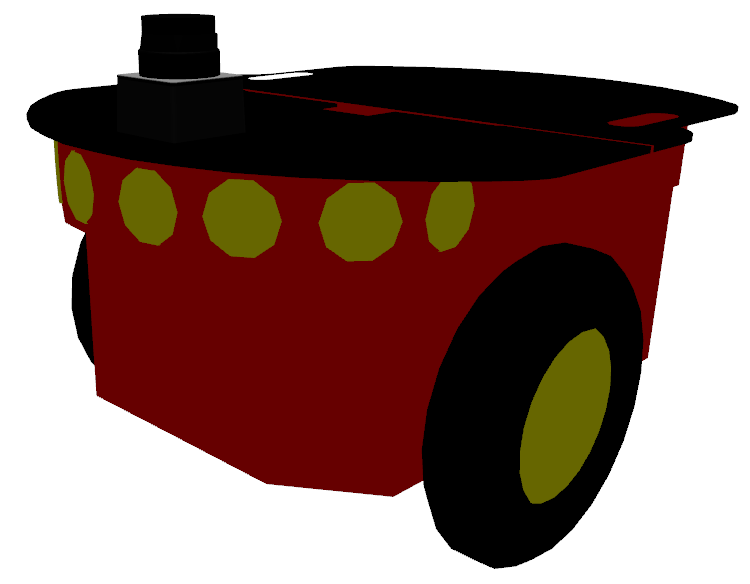
\includegraphics[clip=true, width=0.33\textwidth]{imagenes/pion/sim.png}}

  \caption[Robot diferencial Pioneer 3-DX.]{Robot diferencial Pioneer 3-DX.}\label{fig:p3dx}
   % A la izquierda se muestra el robot real, y a la derecha su versión simulada.

\end{figure}

La flota de exploración se compone de cinco robots ubicados inicialmente en las posiciones
indicadas en la figura \ref{fig:willow}.
% Las comunicaciones entre los robots de
% la flota son sin perdida y de rango infinito.

\subsection{Software}
El software utilizado en las pruebas fue Ubuntu \emph{20.04}, \gls{ROS} \emph{Noetic} y Gazebo
\emph{11.5.1}. 

\subsection{Hardware}
El simulador junto al resto de procesos necesarios para llevar a cabo una
prueba fueron ejecutados en una computadora personal equipada con un procesador
Intel Core i3-9100F, un procesador gráfico GeForce GTX 660 y 16GB de memoria
RAM.

\section{Métricas}
Con el propósito comparar cuantitativamente los resultados de las pruebas se
establece un conjunto de métricas. Estas se describen en los que resta de la
sección. 

Una parte de las métricas utilizadas se proponen en \cite{yan2015metrics} y
evalúan el problema de exploración en general, estas son: \emph{tiempo de
exploración}, \emph{distancia total recorrida por la flota}, \emph{completitud
del mapa} y \emph{calidad del mapa}. 

El \emph{tiempo de exploración} refiere al tiempo que ocurre desde que comienza la
primera asignación de objetivos (sección \ref{sec:asigTar}) hasta que no se
detecta más espacio desconocido por explorar y se da por terminada la
exploración.

La \emph{distancia total recorrida por la flota} es la suma de las distancias
recorridas por cada robot de la flota a lo largo de la exploración. En
\cite{yan2015metrics} esta métrica se presenta como \emph{costo de
exploración}, ya que los autores la consideran como una buena aproximación del
costo energético del robot. 

 % mapas de referencia para evaluar los mapas resultantes de las pruebas,

Para calcular las métricas de \emph{completitud} y \emph{calidad} de los mapas
es necesario contar con mapas de referencia considerados como correctos. En
este proyecto estos se representan a través de grillas de ocupación al igual
que los generados en la exploración. Se definen cuatro mapas de
referencia, uno por cada nivel de granularidad utilizado en las pruebas, con el
propósito de poder comparar cualquiera de los mapas obtenidos en pruebas con
un mapa de referencia de igual granularidad. Los mapas de referencia se pueden
apreciar en la figura \ref{fig:mref}. 

\begin{figure}[H]
  \centerfloat

  \subfloat[$1  \frac{celda}{m^2}$]{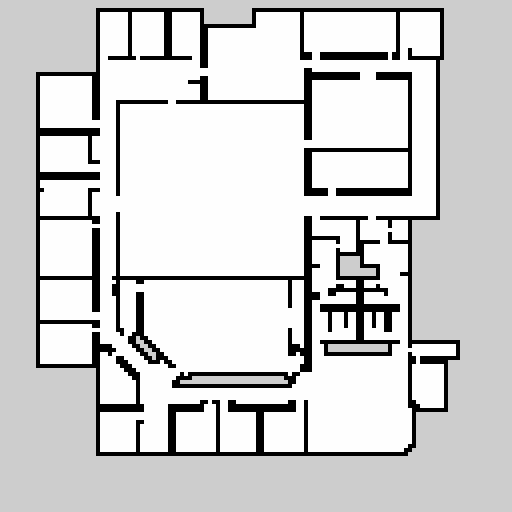
\includegraphics[clip=true, width=0.22\textwidth]{imagenes/willow_ref/1_000000m.png}}
  \qquad
  \subfloat[$4  \frac{celda}{m^2}$]{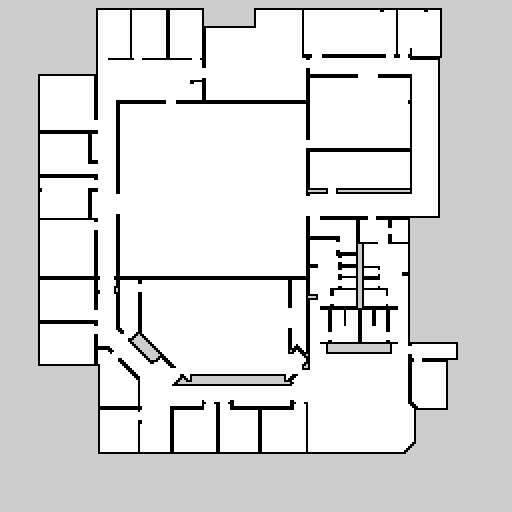
\includegraphics[clip=true, width=0.22\textwidth]{imagenes/willow_ref/0_500000m.png}}
  \qquad
  \subfloat[$9\frac{celda}{m^2}$]{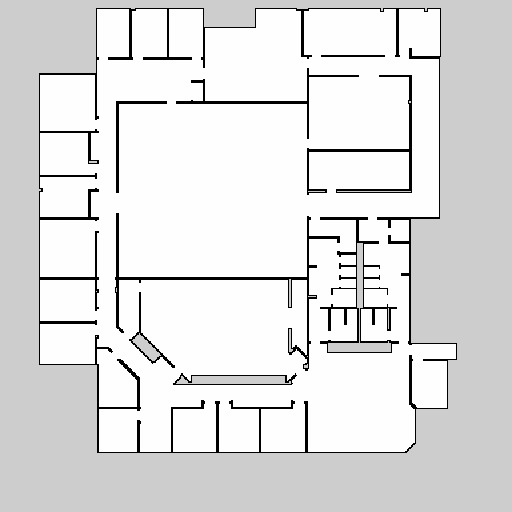
\includegraphics[clip=true, width=0.22\textwidth]{imagenes/willow_ref/0_333333m.png}}
  \qquad
  \subfloat[$16 \frac{celda}{m^2}$]{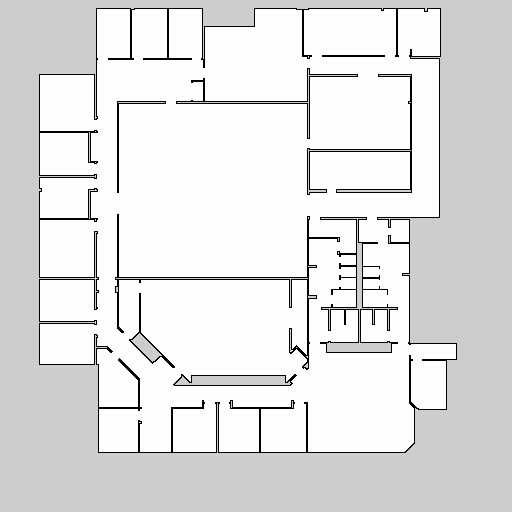
\includegraphics[clip=true, width=0.22\textwidth]{imagenes/willow_ref/0_250000m.png}}

  \caption[Mapas de referencia utilizados.]{Mapas de referencia utilizados. En negro se indican las paredes, en blanco el espacio libre y en gris el espacio desconocido por ser inaccesible.}\label{fig:mref}
   % A la izquierda se muestra el robot real, y a la derecha su versión simulada.

\end{figure}

Notar que existe espacio desconocido en los mapas de referencia, esto se debe a
que las grillas de ocupación no se ajustan al espacio explorable. En términos de
las métricas calculadas, el espacio que es desconocido en los mapas de
referencia no es considerado como parte de los mapas, tanto en los mapas de
referencia como en los obtenidos en las pruebas.

% Es decir las unicas celdas que se consideran como
% parte de los mapas al calcular las metricas son las que tienen un estado
% distinto a desconocido en los mapas de referencia.
% De
% esta forma los mapas de referencia no contienen celdas desconocidas, a
% diferencia de los mapas resultantes de las pruebas los cuales si pueden.

La \emph{completitud del mapa} se define según (\ref{eq:metComp}) donde
$M_{exp}$ es el área conocida del mapa resultante de la exploración y $M_{ref}$
es el área del mapa de referencia.

\begin{equation} \label{eq:metComp}
completitud\ del\ mapa = \frac{M_{exp}}{M_{ref}}
\end{equation}

La \emph{calidad del mapa} se define en (\ref{eq:metCal}) donde se introduce
$E_{exp}$ equivalente al área ocupada por las celdas del mapa resultante de
la exploración cuyo estado difiere del estado de su celda correspondiente en el
mapa de referencia.

\begin{equation} \label{eq:metCal}
calidad\ del\ mapa = \frac{M_{exp}-E_{exp}}{M_{ref}}
\end{equation}

El resto de las métricas fueron diseñadas específicamente para este proyecto,
estas son: \emph{tiempo promedio en construcción de GVD} y \emph{tiempo
promedio en simplificación de fronteras}.

El \emph{tiempo promedio en construcción de GVD} es el tiempo promedio que toma
construir el GVD en la etapa de obtención de información de cada asignación
de objetivos (sección \ref{sec:asigTar}).

El \emph{tiempo promedio en simplificación de fronteras} es el tiempo promedio
que se demora en simplificar las fronteras para identificar los objetivos en
la etapa de obtención de información de cada asignación de objetivos.

\section{Resultados}
\newlength{\graphlen}
\setlength{\graphlen}{0.75\textwidth}


Los resultados experimentales son presentados y analizados en esta
sección. Las tablas que se encuentran a lo largo de la sección indican los
promedios y desviaciones estándar de las métricas obtenidas en las 20
repeticiones que se hacen debido al no determinismo del simulador.

\subsection{Cubrimiento y calidad de los mapas} \label{sec:exp:cubcal}
% Capaz aca puedo mencionar lo que pasa con los errores

% el cubrimiento y la completitud: completitud mayor a 0.999 para todas combinaciones de granularidades y soluciones probadas

% el error y la calidad:

En la tabla \ref{tab:todo3} se muestra la completitud y calidad de los mapas
obtenidos en todas las pruebas realizadas. 

Con respecto a la completitud es posible apreciar que no existen diferencias
mayores entre las variantes de la implementación, teniendo todos los mapas
generados una completitud alta. Dado que el criterio de parada es que no se
detecte más espacio por explorar, estos valores hablan principalmente de la
capacidad de detectar el espacio desconocido explorable que tienen las
soluciones. Todas las soluciones detectan espacio desconocido explorable
mientras exista una un celda $c_1$ libre y otra $c_2$ desconocida tal que $c_1
\in ady_4(c_2)$ (sección \ref{subsec:Grilla}), principalmente porque en estas
condiciones se asume que los robots no pueden atravesar de $c_1$ a $c_2$. Dicho
esto se presume que la completitud de los mapas no es perfecta debido a la
presencia de celdas ubicadas en esquinas de paredes que a pesar de no
cumplir con las condiciones de ser detectadas como explorables, lo son. Un
ejemplo de este tipo de celda se muestra en la figura \ref{fig:faltaCub}. Sin
embargo los valores de completitud obtenidos indican que este tipo de
situaciones son despreciables.

\begin{figure}[H]
  \centerfloat

  \subfloat[Mapa de referencia.]{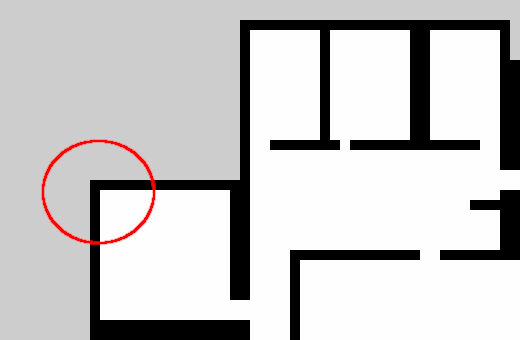
\includegraphics[clip=true, width=0.33\textwidth]{imagenes/faltaDeCub/ogred.png}}
  \qquad
  \subfloat[Mapa generado.]{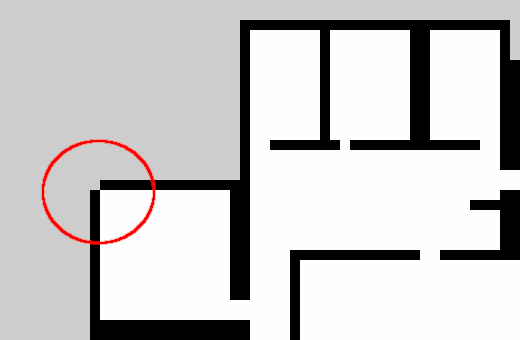
\includegraphics[clip=true, width=0.33\textwidth]{imagenes/faltaDeCub/faltaCubRed}}

  \caption[Celda explorable que no se reconoce como tal.]{Esquina superior izquierda del mapa referencia y de uno de los mapas
  obtenidos en las pruebas que presenta una celda explorable que no se reconoce
como tal. Ambos mapas corresponden a una granularidad de una celda por metro cuadrado.}\label{fig:faltaCub}
   % A la izquierda se muestra el robot real, y a la derecha su versión simulada.

\end{figure}

Los resultados de calidad de los mapas obtenidos son similares a los de
completitud, los mapas construidos tienen una calidad alta, sin existir
diferencias significativas entre las variantes. Esto es esperable ya que
los sensores simulados fueron configurados para proporcionar medidas perfectas.
Aunque a pesar de esto la calidad de los mapas no perfecta, esto puede explicarse en primer
lugar por el impacto de la completitud del mapa en su calidad. En segundo lugar
por la existencia de varios robots que pueden detectase como obstáculos entre
sí, generado celdas obstaculizadas que no se encuentran en el mapa de
referencia. Y en tercer lugar porque a pesar de la configuración de los
sensores, estos proporcionan medidas con un ruido pequeño.

Estos resultados de completitud y calidad del mapa permiten concluir que todas
las variantes logran resolver de manera satisfactoria el problema de
exploración multi-robot en términos de los mapas construidos. Las
siguientes secciones se dedican a discutir el impacto de las diferentes
variantes en términos de tiempo y costo de exploración.


\begin{table}[H]
%29/12/2021 18:15:43
\hbadness = 10000
\tolerance=9999
\emergencystretch=10pt
\hyphenpenalty=10000
\exhyphenpenalty=100
\begin{center}

% \begin{adjustbox}{minipage=0.75\paperwidth, center}
\begin{adjustbox}{width=1\textwidth}
\small

\begin{tabularx}{\textwidth}{|X|C{0.80cm}|X|X|}

\hline
Variante & $\frac{celdas}{m^2}$ & Completitud del mapa & Calidad del mapa \\ \hline\hline
\multirow{4}{\linewidth}{\centering Propuesta sin cambios}
& 1 & 0.999725±1.5e-04 & 0.999039±3.1e-04\\ \cline{2-4}
& 4 & 0.999925±6.5e-05 & 0.999703±1.7e-04\\ \cline{2-4}
& 9 & 0.999983±1.2e-05 & 0.999858±5.7e-05\\ \cline{2-4}
& 16 & 0.999998±3.6e-06 & 0.999929±3.4e-05\\ \hline\hline
\multirow{4}{\linewidth}{\centering No incremental}
& 1 & 0.999763±8.9e-05 & 0.999208±2.2e-04\\ \cline{2-4}
& 4 & 0.999957±4.2e-05 & 0.999805±1.3e-04\\ \cline{2-4}
& 9 & 0.999984±1.6e-05 & 0.999864±4.7e-05\\ \cline{2-4}
& 16 & 0.999999±1.9e-06 & 0.999941±3.3e-05\\ \hline\hline
\multirow{4}{\linewidth}{\centering Simplificación de fronteras basada en K-Means}
& 1 & 0.999802±1.3e-04 & 0.999179±2.8e-04\\ \cline{2-4}
& 4 & 0.999977±2.7e-05 & 0.999767±8.0e-05\\ \cline{2-4}
& 9 & 0.999976±2.3e-05 & 0.999831±7.4e-05\\ \cline{2-4}
& 16 & 0.999999±2.5e-06 & 0.999930±1.8e-05\\ \hline\hline
\multirow{4}{\linewidth}{\centering Fronteras sin simplificar}
& 1 & 0.999937±7.6e-05 & 0.999493±2.0e-04\\ \cline{2-4}
& 4 & 0.999995±9.8e-06 & 0.999837±4.8e-05\\ \cline{2-4}
& 9 & 0.999983±4.0e-05 & 0.999729±7.6e-05\\ \cline{2-4}
& 16 & 0.999998±4.1e-06 & 0.999921±2.2e-05\\ \hline\hline
\multirow{4}{\linewidth}{\centering Desconocidas se consideran libres}
& 1 & 0.999812±1.1e-04 & 0.999256±3.2e-04\\ \cline{2-4}
& 4 & 0.999972±1.9e-05 & 0.999786±9.7e-05\\ \cline{2-4}
& 9 & 0.999987±1.2e-05 & 0.999840±6.9e-05\\ \cline{2-4}
& 16 & 0.999998±3.5e-06 & 0.999940±2.8e-05\\ \hline
\end{tabularx}
\end{adjustbox}

\caption{Completitud y calidad de los mapas obtenidos en todas las pruebas realizadas.}
\label{tab:todo3}
\end{center}

\end{table}


\subsection{Incrementalidad}\label{sec:exp:inc}
En esta sección se comparan los resultados de las pruebas realizadas con la
solución propuesta que construye el GVD de forma incremental, contra los de la 
variante que solo difiere en que la construcción del GVD es no incremental. Las
métricas analizadas en esta sección se encuentran en la tabla \ref{tab:inc1}
y graficadas en las figuras \ref{fig:gra:inc:et}, \ref{fig:gra:inc:ec} y
\ref{fig:gra:inc:gvdt}.

En cada nivel de granularidad la variante incremental reduce en un
${\smallsim}94\%$ el tiempo promedio construcción del GVD con respecto a la
variante no incremental. Esto valida la idea de que la construcción incremental
del GVD es más eficiente que su contraparte no incremental.

% El tiempo de construcción de GVD impacta directamente al tiempo que ocurre
% desde que un robot pide un objetivo y una le es asignada, ya que es una parte
% necesaria y no paralelizada de la etapa de obtención de información (sección
% \ref{subsec:obtInfo}) de cada asignación de objetivos (sección \ref{sec:asigTar}).
% A pesar de esto el impacto sobre los tiempos de exploración no es directo. Esto
% se debe al hecho de que una asignación de objetivos este en curso solo asegura que un único
% robot estara osicoso, ya que mientras que un robot pide una objetivo y la obitene
% el resto puede estar completando objetivos asignadas previamente. Cuanto más corta 
% es la demora en la asignación de objetivos más probable es que un único robot quede
% osicoso, mientras que si dicha demora aumenta, también lo hace la probabilidad
% que en el transcurso de la asignacion más robots completen sus objetivos y
% requieran objetivos, quedando ociosos. Esto logra explicar que en todos los
% niveles de granularidad la reduccion del tiempo promedio logrado por la
% variante incremental frente a la no incremental sea de un ${\smallsim}94\%$
% constante mientras que la reduccion del tiempo de exploración comienza siendo
% de un ${\smallsim}8\%$ en el nivel de granularidad más bajo (tiempos de
% construcción de GVD más altos), creciendo mediante se aumenta el nivel de
% granularidad llegando a una reduccion de un ${\smallsim}63\%$ en la
% granularidad más alta (tiempos de construcción de
% GVD más altos).

Con respecto a los tiempos de exploración, estos también son reducidos al
construir el GVD de forma incremental. La reducción comienza siendo de
${\smallsim}8\%$ en el nivel de granularidad más bajo, y mediante se aumenta el
nivel de granularidad las reducciones también aumentan hasta llegar a una
reducción de ${\smallsim}63\%$ en el nivel más alto. Esto se explica porque el
tiempo de construcción de GVD impacta directamente al tiempo que ocurre desde
que un robot pide un objetivo y uno le es asignado, por ser una parte necesaria y
no paralelizada de la etapa de obtención de información (sección
\ref{subsec:obtInfo}) de cada asignación de objetivos (sección
\ref{sec:asigTar}). Y a su vez los tiempos de asignación de objetivos impactan
a los tiempos de exploración, pero en este caso el impacto no es directo. Esto
se debe a que el hecho de que exista una asignación de objetivos en curso solo
asegura que un único robot está ocioso, porque mientras que un robot pide un
objetivo y uno le es asignado el resto puede estar completando objetivos que le
fueron asignados previamente. Cuanto más corta sea la demora en la asignación
de objetivos más probable es que un único robot quede ocioso, mientras que si
dicha demora aumenta, también lo hace la probabilidad de que en el transcurso de
la asignación más robots completen sus objetivos y requieran nuevos objetivos,
quedando ociosos. 
% no son
% monótonamente crecientes ni decrecientes respecto a la granularidad

% las reducciones no son significativas. Especificamente, 
% y adicionalmente las diferencias entre los promedios de
% esta metrica son similares a sus desviaciones estándar

Construir el GVD de forma incremental también parece reducir las distancias
totales recorridas por la flota en todas las granularidades, aunque en este
caso las reducciones están comprendidas entre $2\%$ y $7\%$, fluctuando al
aumentar los niveles de granularidad. Esto puede deberse a que tiempos más
rápidos de asignación de objetivos hacen más probable que los robots cambien su
trayectoria a un nuevo objetivo antes de llegar a la ubicación exacta del
objetivo previamente completado. Esto puede reducir la distancia recorrida por
el robot si los caminos hacia el objetivo anterior y el actual no se solapan.

% En cada nivel de granularidad el tiempo promedio en construcción del GVD de
% variante incremental siempre es menor que el de la variante no incremental,
% aumentando la diferencia a medida que aumentan las celdas por metro cuadrado.
% La reducción del tiempo tiempo de construcción del GVD que se logra al

% construirlo de forma incremental implica una reducción del $55\%$ en el
% porcentaje de tiempo de la obtención de información en la que se construye el
% GVD aproximadamente que se repite en todos los niveles de granularidad.

% Como los tiempos de construcción promedio del GVD son menores
% en las pruebas realizadas con las construcción incremental del GVD,

% al aumentar las celdas por metro cuadrado, el tiempo
% promedio en construcción del GVD, en el caso de la construcción incremental crece de a 

\begin{table}[H]
%29/12/2021 18:15:42
\hbadness = 10000
\tolerance=9999
\emergencystretch=10pt
\hyphenpenalty=10000
\exhyphenpenalty=100
\begin{center}

% \begin{adjustbox}{minipage=0.75\paperwidth, center}
\begin{adjustbox}{width=1\textwidth}
\small

\begin{tabularx}{\textwidth}{|X|C{0.80cm}|X|X|X|}

\hline
Construcción del GVD & $\frac{celdas}{m^2}$ & Tiempo de exploración $(s)$ & Distancia total recorrida por la flota $(m)$ & Tiempo promedio en construcción de GVD $(s)$ \\ \hline\hline
\multirow{4}{\linewidth}{\centering Incremental}
& 1 & 463.0±22.6 & 2480.5±109.7 & 0.0442±0.0017\\ \cline{2-5}
& 4 & 496.4±19.0 & 2745.2±107.3 & 0.1762±0.0057\\ \cline{2-5}
& 9 & 549.2±18.4 & 2849.3±95.2 & 0.4204±0.0174\\ \cline{2-5}
& 16 & 678.4±24.8 & 3050.3±105.2 & 0.7641±0.0334\\ \hline\hline
\multirow{4}{\linewidth}{\centering No incremental}
& 1 & 501.9±22.4 & 2653.4±96.5 & 0.7199±0.0122\\ \cline{2-5}
& 4 & 745.7±23.1 & 2851.1±144.0 & 2.8603±0.0484\\ \cline{2-5}
& 9 & 1198.7±35.8 & 3038.1±159.2 & 6.8253±0.1713\\ \cline{2-5}
& 16 & 1856.7±56.2 & 3117.0±170.3 & 12.9256±0.3056\\ \hline
\end{tabularx}
\end{adjustbox}

\caption{Resultados obtenidos en las pruebas realizadas con la construcción incremental y no incremental del GVD.}
\label{tab:inc1}
\end{center}

\end{table}
\todo[inline]{cuadro 4.2: qué tal, Construcción del GVD: incremental vs no incremental}



\begin{figure}[H]
  \centerfloat

  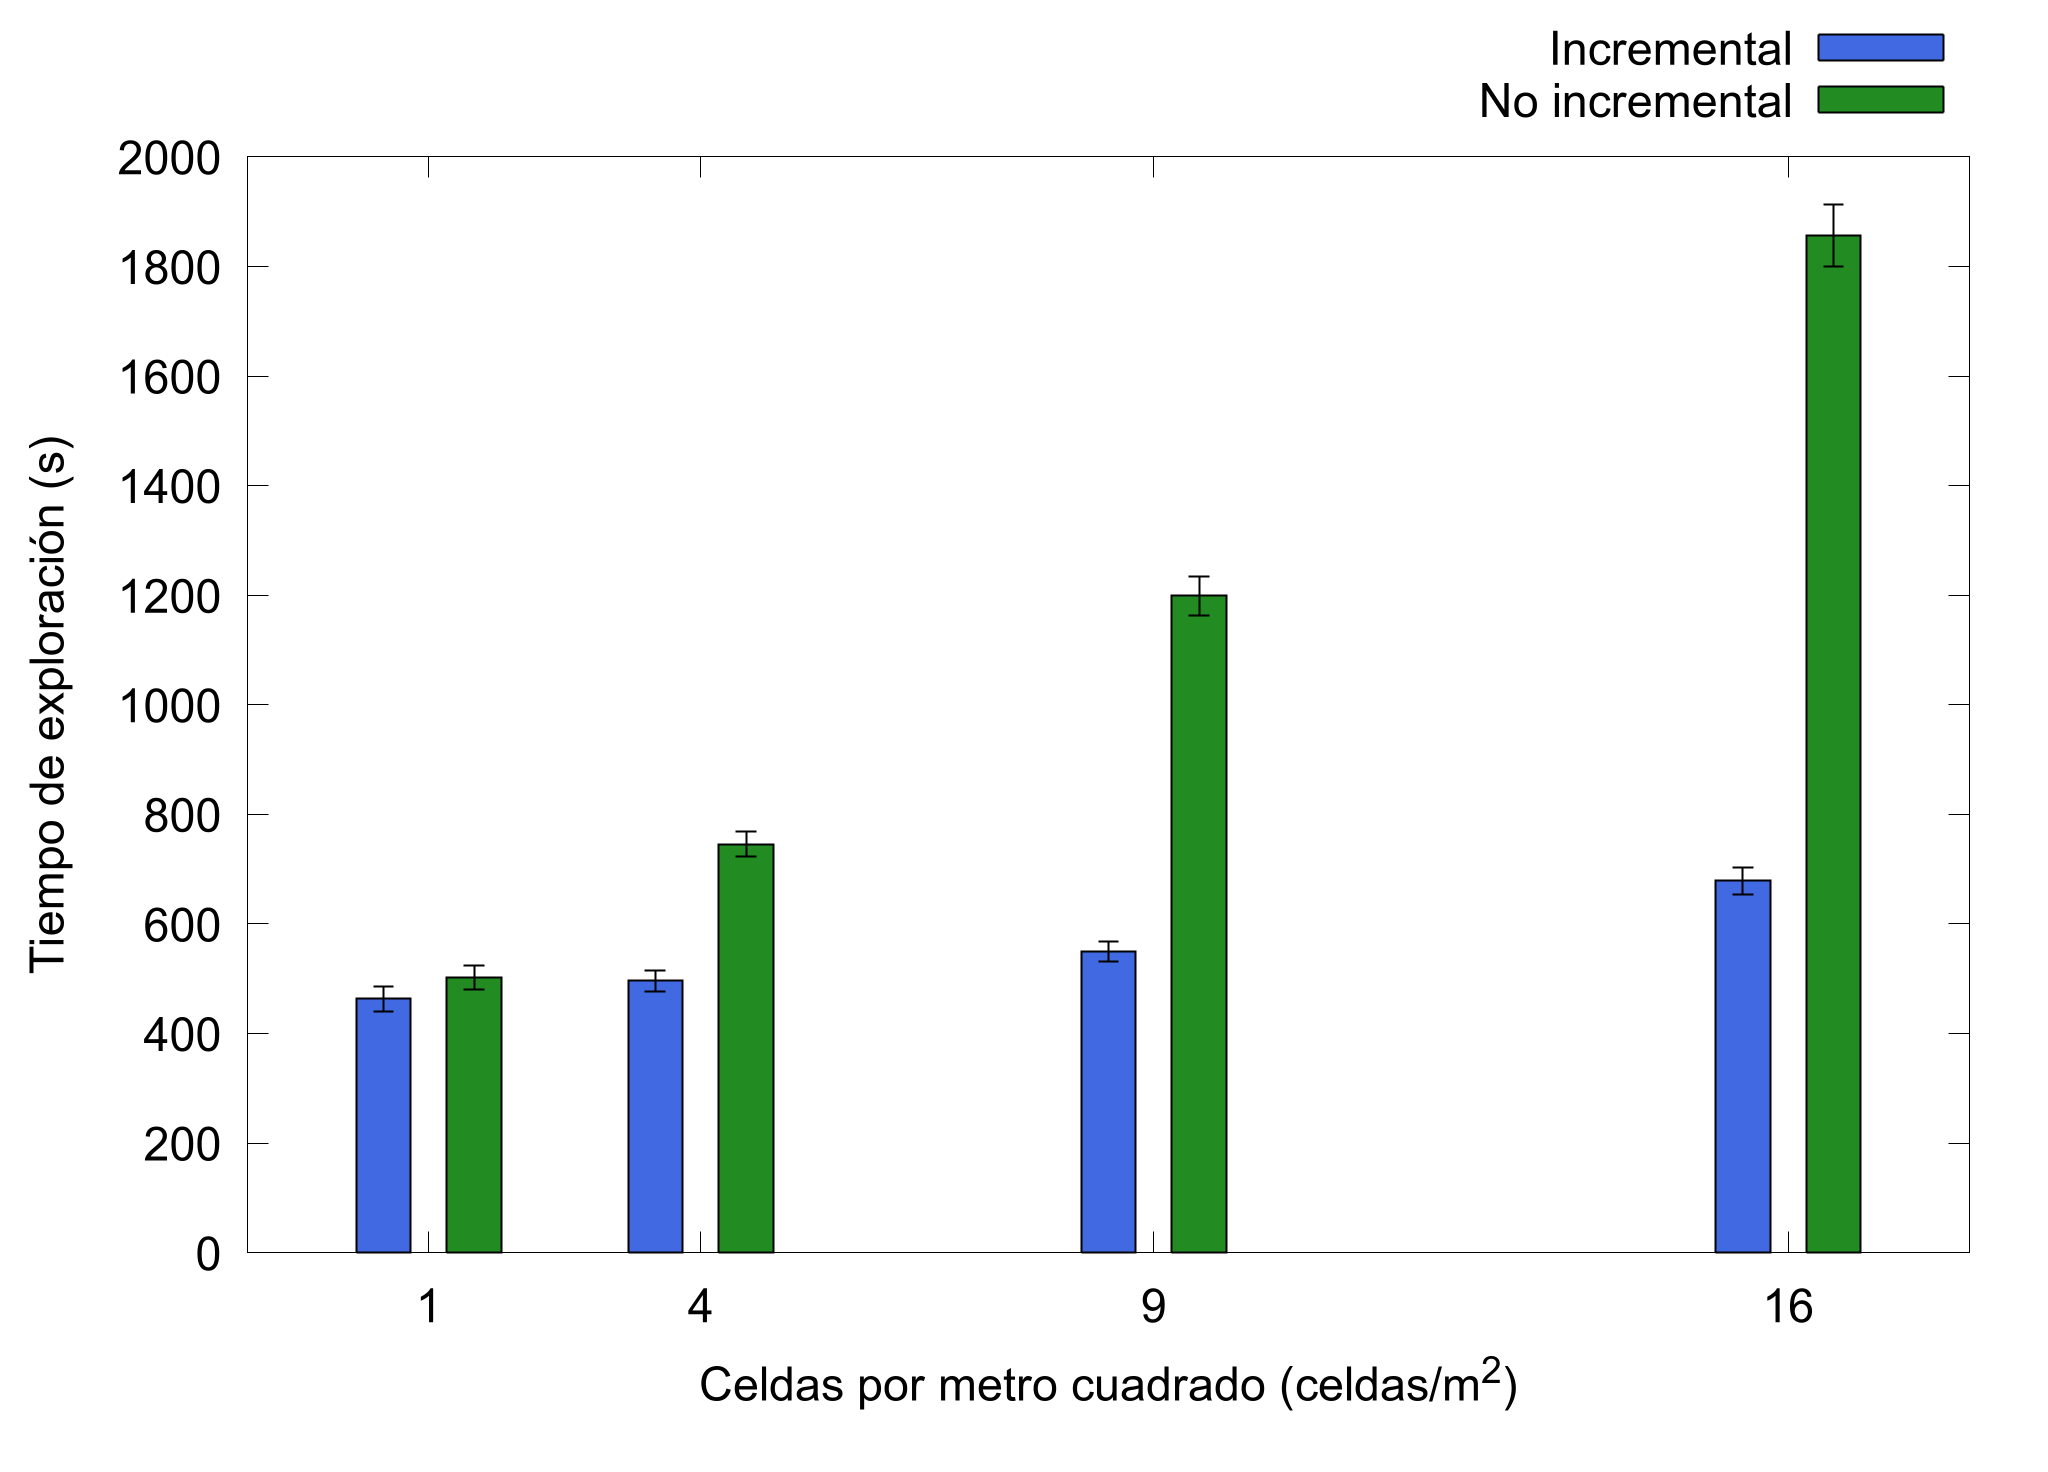
\includegraphics[clip=true, width=\graphlen]{imagenes/graficas_chicas/graficas_histo_num/incrementalidad/exploration_time.png}

  \caption{Tiempo de exploración en función de celdas por metro cuadrado.}\label{fig:gra:inc:et}

\end{figure}

\begin{figure}[H]
  \centerfloat

  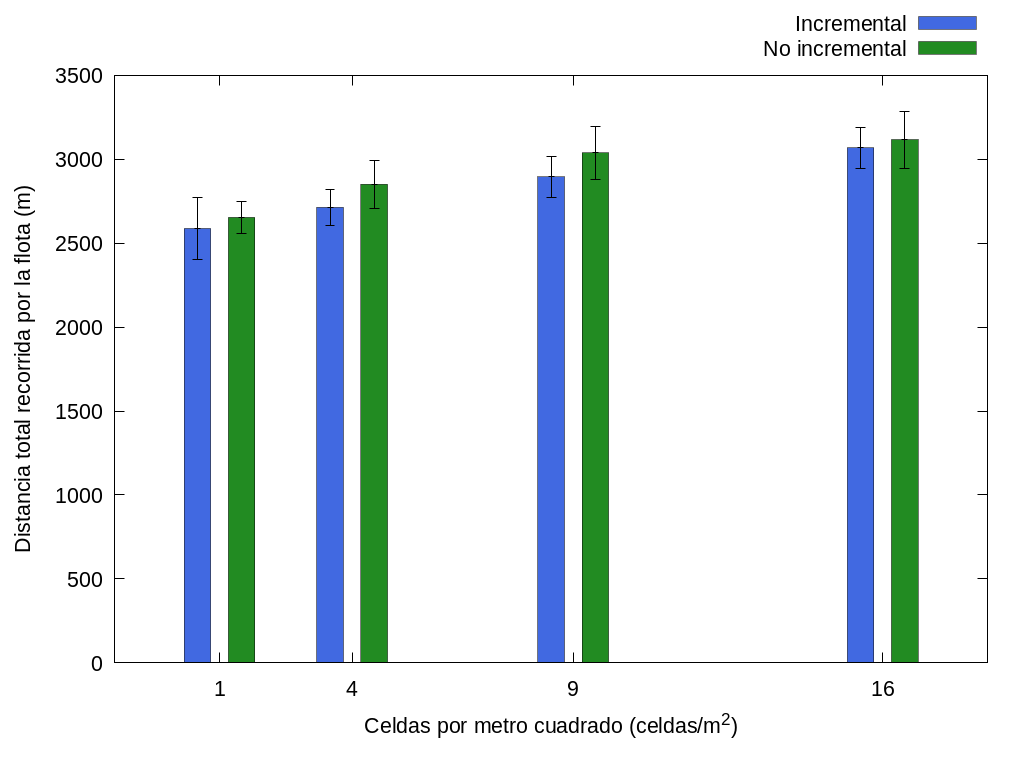
\includegraphics[clip=true, width=\graphlen]{imagenes/graficas_chicas/graficas_histo_num/incrementalidad/exploration_cost.png}

  \caption{Distancia total recorrida por la flota  en función de celdas por metro cuadrado.}\label{fig:gra:inc:ec}

\end{figure}

\begin{figure}[H]
  \centerfloat

  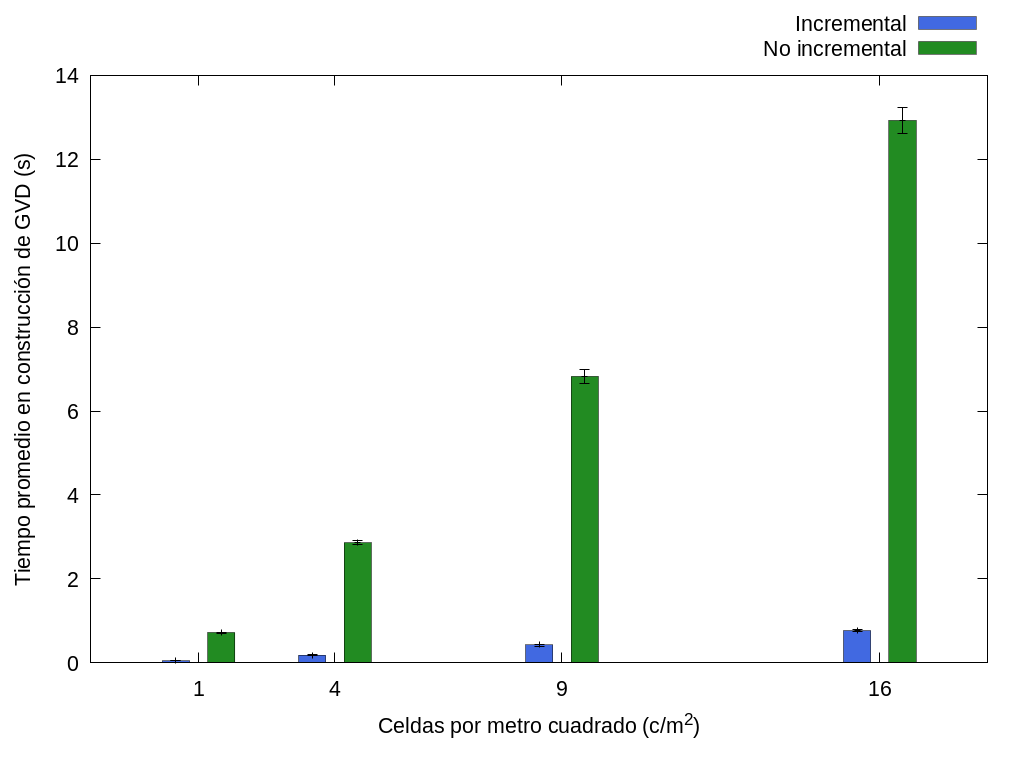
\includegraphics[clip=true, width=\graphlen]{imagenes/graficas_chicas/graficas_histo_num/incrementalidad/gvd_construction_time_mean.png}

  \caption{Tiempo promedio en construcción de GVD en función de celdas por metro cuadrado.}\label{fig:gra:inc:gvdt}

\end{figure}


\subsection{Identificación de objetivos}\label{sec:exp:idobj}
En esta sección se realiza un análisis comparativo de los resultados obtenidos
en pruebas realizadas con tres soluciones distintas que difieren únicamente en
el método usado para identificar objetivos (sección \ref{sec:pc:idobj}). Estos
métodos son: la simplificación de fronteras basada en cubrimiento propuesta en
este proyecto, simplificación de fronteras basada en K-Means como es utilizada en
\cite{Amorin2019} y la identificación de fronteras (sin simplificar)
introducida en \cite{yamauchi1998frontier}. Los resultados de las métricas
analizadas en esta sección se presentan en la tabla \ref{tab:ident_obj1} y se encuentran graficadas en
las figuras \ref{fig:gra:idobj:et}, \ref{fig:gra:idobj:ec} y
\ref{fig:gra:idobj:iobt}.

Es posible apreciar que los métodos que identifican los objetivos simplificando
las fronteras reducen los tiempos de exploración con respecto al método que
identifica a las fronteras sin simplificar como objetivos. Aunque en el nivel
de granularidad más bajo las reducciones son menores a ${\smallsim}5\%$, estas crecen junto
a la granularidad hasta alcanzarse una reducción de ${\smallsim}29\%$ en el
nivel más alto. Esto puede deberse al tiempo de asignación de objetivos como se
explica en la sección \ref{sec:exp:inc}. En este caso se considera que los
factores con mayor impacto sobre los tiempos de asignación de objetivos son dos:
el tiempo de simplificación de fronteras y la cantidad de objetivos
identificados. Mayores tiempos de simplificación fronteras retrasan la
identificación de objetivos, parte necesaria y no paralelizada de la etapa de
obtención de información (sección \ref{subsec:obtInfo}) en la asignación de
objetivos. Mientras que disminuir la cantidad de objetivos identificados implica
reducciones en la duración de las etapas de valuación (sección
\ref{subsec:MiValSub}) y de resolución (sección \ref{subsec:MiResSub}) al ser
menor la cantidad de objetivos a valuar y a considerar en la resolución. Entonces lo que se evidencia
en los resultados obtenidos, es que invertir tiempo en disminuir los objetivos
identificados simplificando las fronteras lleva a una reducción total de los
tiempos de asignación de objetivos, y en consecuencia de los tiempos de exploración
frente a no invertir dicho tiempo y utilizar todas las fronteras sin
simplificar. Otra razón posible para las reducciones del tiempo de exploración
es que simplificar las fronteras puede aportar a la coordinación de los robots.
Por ejemplo de no simplificarse las fronteras se permite que un robot sea
asignado a un objetivo adyacente a una pared o que dos robots sean asignados a
objetivos adyacentes entre sí, situaciones en las cuales se desaprovecha
capacidad de sensado, y se complejiza la navegación. Al simplificarse las
fronteras, especialmente cuando se logra el cubrimiento minimizando los
objetivos resultantes, se evitan situaciones como las descritas lo cual puede
verse como una coordinación pasiva. \todo{o implicita?}

De acuerdo con los resultados simplificar las fronteras en la identificación de
objetivos también reduce las distancias totales recorridas por la flota frente
a no simplificarlas. Estas reducciones son en general de ${\smallsim}10\%$, y
pueden ser causadas por la disminución del tiempo de asignación de objetivos,
debido a las mismas razones que se explican en la sección \ref{sec:exp:inc}.
Aunque la coordinación pasiva también puede estar jugando un rol al evitar que
los robots se trasladen a objetivos que desaprovechan sus capacidades
sensoriales o que puedan llevar a inconvenientes en la navegación.

Con respecto a los dos métodos que simplifican las fronteras para 
identificar objetivos, en el nivel de granularidad más bajo, la
simplificación basada en cubrimiento logra reducciones con respecto a la
basada en K-Means de ${\smallsim}3\%$ en las distancias totales recorridas por la
flota y de ${\smallsim}5\%$ en los tiempos de exploración. Esto se invierte a
medida que aumenta el nivel de granularidad, hasta que en el nivel más alto en
lugar de reducirse, las métricas aumentan. Las distancias totales recorridas por la
flota aumentan en un ${\smallsim}3\%$ y los tiempos de exploración en un
${\smallsim}6\%$. Por otro lado según los tiempos
promedio en simplificación de fronteras, la simplificación basada en
cubrimiento en todo nivel de granularidad es entre $2$ y
$4$ veces más lenta que la basada en K-Means. Estos resultados
parecen indicar que la simplificación basada en cubrimiento toma más tiempo
pero logra mejores reducciones de objetivos que la basada en K-Means. En el
nivel de granularidad más bajo el aumento de tiempo de simplificación no es tan
relevante como la reducción de objetivos, por lo tanto la simplificación basada
en cubrimiento obtiene un mejor rendimiento. A medida la granularidad crece el
aumento de tiempo de simplificación se torna más relevante que la reducción de
objetivos, por lo que la simplificación basada en K-Means obtiene un
rendimiento superior.  

\begin{table}[H]
%24/12/2021 03:06:43
\hbadness = 10000
\tolerance=9999
\emergencystretch=10pt
\hyphenpenalty=10000
\exhyphenpenalty=100
\begin{center}

% \begin{adjustbox}{minipage=0.75\paperwidth, center}
\begin{adjustbox}{width=1\textwidth}
\small

\begin{tabularx}{\textwidth}{|X|C{0.80cm}|X|X|}

\hline
Identificación de objetivos & $\frac{celdas}{m^2}$ & Tiempo de exploración $(s)$ & Distancia total recorrida por la flota $(m)$ \\ \hline\hline
\multirow{4}{\linewidth}{\centering Simplificación de fronteras basada en cubrimiento}
& 1 & 480.8±34.7 & 2587.0±186.4\\ \cline{2-4}
& 4 & 498.0±25.3 & 2713.1±107.5\\ \cline{2-4}
& 9 & 553.4±24.9 & 2894.7±124.5\\ \cline{2-4}
& 16 & 689.7±29.0 & 3067.9±121.9\\ \hline\hline
\multirow{4}{\linewidth}{\centering Simplificación de fronteras basada en K-Means}
& 1 & 491.0±25.7 & 2628.0±98.6\\ \cline{2-4}
& 4 & 494.3±28.2 & 2684.8±106.7\\ \cline{2-4}
& 9 & 532.6±21.1 & 2813.0±96.4\\ \cline{2-4}
& 16 & 652.0±32.7 & 2962.4±136.6\\ \hline\hline
\multirow{4}{\linewidth}{\centering Fronteras sin simplificar}
& 1 & 487.9±24.3 & 2750.7±142.3\\ \cline{2-4}
& 4 & 532.8±24.7 & 3028.3±136.1\\ \cline{2-4}
& 9 & 643.3±22.8 & 3216.9±121.3\\ \cline{2-4}
& 16 & 925.8±104.7 & 3352.5±208.7\\ \hline
\end{tabularx}
\end{adjustbox}

\caption{Resultados de tiempo y costo de exploración obtenidos en las pruebas realizadas con los distintos métodos de identificación de objetivos.}
\label{tab:ident_obj1}
\end{center}

\end{table}


\begin{figure}[H]
  \centerfloat

  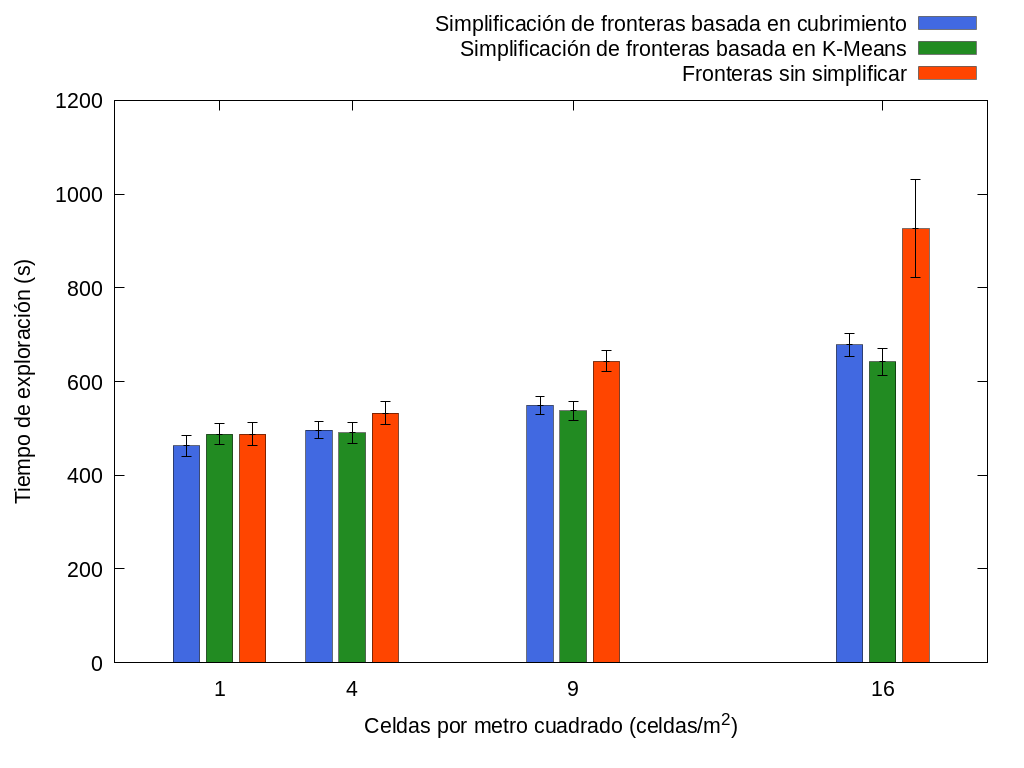
\includegraphics[clip=true, width=\graphlen]{imagenes/graficas_chicas/graficas_histo_num/ident_obj/exploration_time.png}

  \caption{Tiempo de exploración en función de celdas por metro cuadrado.}\label{fig:gra:idobj:et}

\end{figure}

\begin{figure}[H]
  \centerfloat

  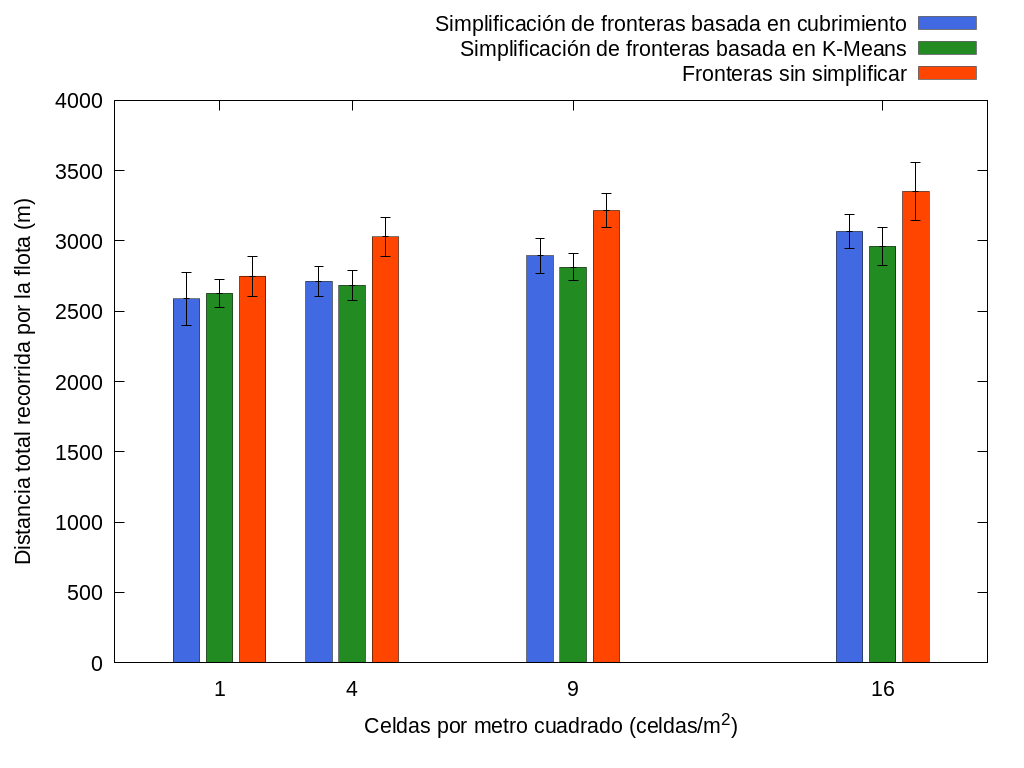
\includegraphics[clip=true, width=\graphlen]{imagenes/graficas_chicas/graficas_histo_num/ident_obj/exploration_cost.png}

  \caption{Distancia total recorrida por la flota en función de celdas por metro cuadrado.}\label{fig:gra:idobj:ec}

\end{figure}

\begin{figure}[H]
  \centerfloat

  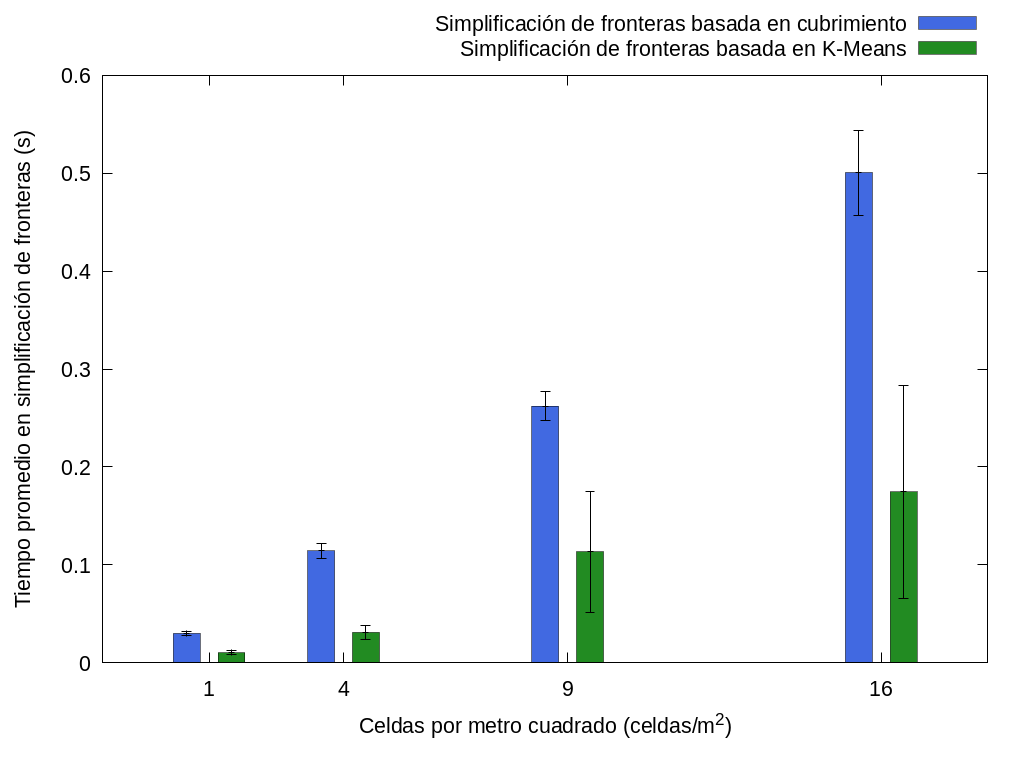
\includegraphics[clip=true, width=\graphlen]{imagenes/graficas_chicas/graficas_histo_num/ident_obj/obj_id_time_mean.png}

  \caption{Tiempo promedio en obtención de información función de celdas por metro cuadrado.}\label{fig:gra:idobj:iobt}

\end{figure}

\subsection{Consideración del espacio desconocido}\label{sec:exp:desco}

% T
% t
Las pruebas analizadas en esta sección corresponden a las realizadas con
soluciones que varían únicamente en la forma de considerar el espacio
desconocido al construir el GVD. Dichas formas son dos: considerar las
celdas desconocidas como libres y considerar que las celdas desconocidas no
propagan ondas y que el conjunto $\mli{UF}$ de celdas desconocidas que son
adyacentes a celdas libres pertenecen a generadores ($\mli{UF} \subseteq
\mli{CGen}$). Ambas formas son descritas en la sección \ref{subsec:espDesc}. Los
resultados obtenidos en estas pruebas se presentan en la tabla \ref{tab:desconocido1} y sus
gráficas en las figuras \ref{fig:gra:des:et}, \ref{fig:gra:des:ec} y
\ref{fig:gra:des:gvdt}.

Considerar que las celdas desconocidas no propagan ondas y que $\mli{UF}
\subseteq \mli{CGen}$ logra una reducción de ${\smallsim}61\%$ en el tiempo
promedio de construcción del GVD en cada nivel de granularidad respecto a
considerar a las celdas desconocidas como libres. Estos resultados validan que
restringir la construcción del GVD al espacio conocido lleva a mejoras en los
tiempos de construcción del GVD. 


Adicionalmente tanto el tiempo de exploración como las distancias totales
recorridas por las flota son reducidas al considerar que las celdas
desconocidas no propagan ondas y que $\mli{UF} \subseteq \mli{CGen}$. La
reducción del tiempo de exploración comienza siendo de ${\smallsim}3\%$ en el
nivel de granularidad más bajo, llegando a una reducción de ${\smallsim}29\%$
en el nivel más alto. Mientras que la reducción de la distancia total recorrida
por la flota fluctúa entre ninguna reducción y una reducción de
${\smallsim}9\%$. Esto puede ser causado porque la reducción de los tiempos de
construcción del GVD implica una reducción en los tiempos de asignación de
objetivos que se asocia a reducciones en los tiempos de exploración y de
las distancias totales recorridas por la flota, como se explica en la sección
\ref{sec:exp:inc}. Aunque en este caso las reducciones de los tiempos de construcción del
GVD son menores y por lo tanto los efectos sobre las métricas son menos
pronunciados. A su vez, considerar el espacio desconocido de distinta manera
cambia significativamente la forma del GVD lo cual también puede afectar a los
caminos que los robots generan a partir del GVD y por lo tanto a las métricas en cuestión.


%% donde se compara la construcción incremental y no incremental del GVD
% Con respecto a los tiempos de exploración, estos tambien son reducidos al
% contruir el GVD de forma incremental. La reducción comienza siendo de un
% ${\smallsim}8\%$ en el nivel de granularidad más bajo, y mediante se aumenta el
% nivel de granularidad las reducciones tambien aumentan hasta llegar a una
% reducción de ${\smallsim}63\%$ en el nivel más alto. Esto se explica porque el
% tiempo de construcción de GVD impacta directamente al tiempo que ocurre desde
% que un robot pide un objetivo y una le es asignada, por ser una parte necesaria y
% no paralelizada de la etapa de obtención de información (sección
% \ref{subsec:obtInfo}) de cada asignación de objetivos (sección \ref{sec:asigTar}).
% Y los tiempos de asignación de objetivos impactan a los tiempos de exploración,
% pero en este caso el impacto no es directo. Esto se debe a que una asignación
% de objetivos en curso solo asegura que un único robot esta osicoso, porque
% mientras que un robot pide una objetivo y una le es asignada el resto puede estar
% completando objetivos asignadas previamente. Cuanto más corta es la demora en la
% asignación de objetivos más probable es que un único robot quede osicoso, mientras
% que si dicha demora aumenta, también lo hace la probabilidad que en el
% transcurso de la asignacion más robots completen sus objetivos y requieran objetivos,
% quedando ociosos. 
% no son
% monótonamente crecientes ni decrecientes respecto a la granularidad

% las reducciones no son significativas. Especificamente, 
% y adicionalmente las diferencias entre los promedios de
% esta metrica son similares a sus desviaciones estándar

% Construir el GVD de forma incremental también parece reducir las distancias
% totales recorridas por la flota en todas las granularidades, aunque en este
% caso las reducciones estan comprendidas entre $2\%$ y $7\%$, fluctuando al
% aumentar los niveles de granularidad. Esto puede deberse a que tiempos más
% rapidos de asignación de objetivos hacen más probable que los robots cambien su
% trayectoria a un nuevo objetivo antes de llegar a la ubicación exacta del
% objetivo previamente completado. Esto puede reducir la distancia recorrida por
% el robot si los caminos hacia el objetivo anterior y el actual no se solapan.




\begin{table}[H]
%24/12/2021 03:06:43
\hbadness = 10000
\tolerance=9999
\emergencystretch=10pt
\hyphenpenalty=10000
\exhyphenpenalty=100
\begin{center}

% \begin{adjustbox}{minipage=0.75\paperwidth, center}
\begin{adjustbox}{width=1\textwidth}
\small

\begin{tabularx}{\textwidth}{|X|C{0.80cm}|X|X|}

\hline
Consideración del espacio desconocido & $\frac{celdas}{m^2}$ & Tiempo de exploración $(s)$ & Distancia total recorrida por la flota $(m)$ \\ \hline\hline
\multirow{4}{\linewidth}{\centering Desconocidas no propagan olas y $UF \subseteq CGen$}
& 1 & 480.8±34.7 & 2587.0±186.4\\ \cline{2-4}
& 4 & 498.0±25.3 & 2713.1±107.5\\ \cline{2-4}
& 9 & 553.4±24.9 & 2894.7±124.5\\ \cline{2-4}
& 16 & 689.7±29.0 & 3067.9±121.9\\ \hline\hline
\multirow{4}{\linewidth}{\centering Desconocidas se consideran libres}
& 1 & 479.1±34.4 & 2522.2±149.5\\ \cline{2-4}
& 4 & 510.5±27.1 & 2728.9±135.2\\ \cline{2-4}
& 9 & 677.8±26.4 & 3134.2±148.8\\ \cline{2-4}
& 16 & 955.4±42.1 & 3303.6±240.5\\ \hline
\end{tabularx}
\end{adjustbox}

\caption{Resultados de tiempo y costo de exploración obtenidos en las pruebas realizadas con las distintas consideraciones del espacio desconocido al construir el GVD.}
\label{tab:desconocido1}
\end{center}

\end{table}


\begin{figure}[H]
  \centerfloat

  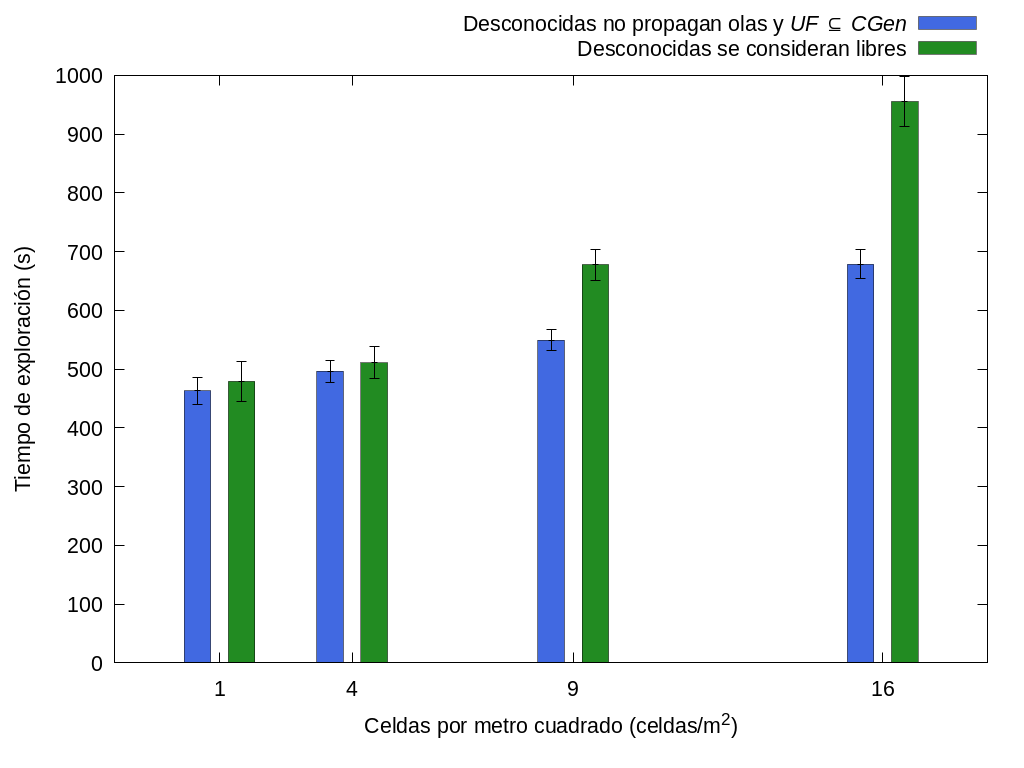
\includegraphics[clip=true, width=\graphlen]{imagenes/graficas_chicas/graficas_histo_num/desconocido/exploration_time.png}

  \caption{Tiempo de exploración en función de celdas por metro cuadrado.}\label{fig:gra:des:et}

\end{figure}

\begin{figure}[H]
  \centerfloat

  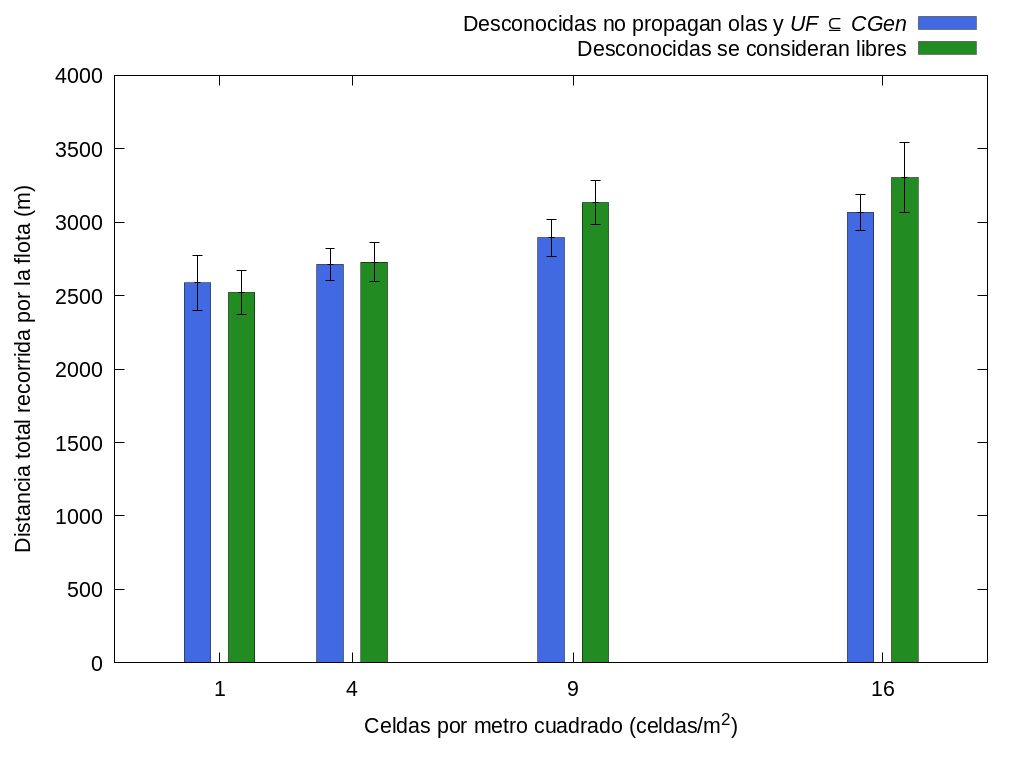
\includegraphics[clip=true, width=\graphlen]{imagenes/graficas_chicas/graficas_histo_num/desconocido/exploration_cost.png}

  \caption{Distancia total recorrida por la flota en función de celdas por metro cuadrado.}\label{fig:gra:des:ec}

\end{figure}

\begin{figure}[H]
  \centerfloat

  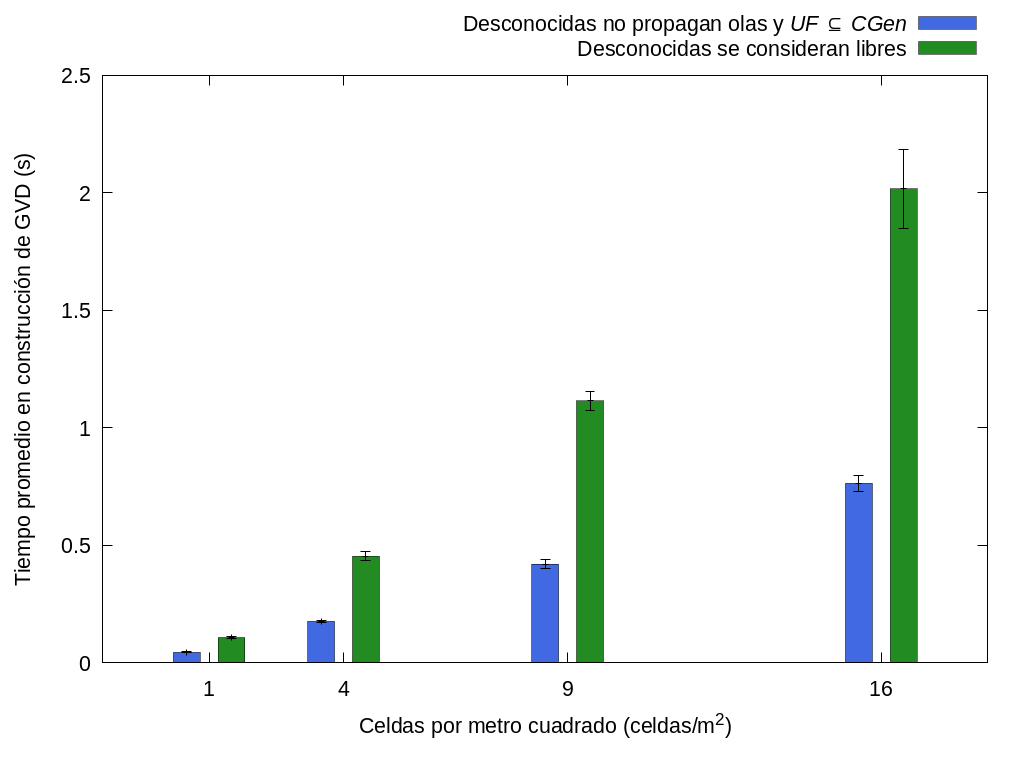
\includegraphics[clip=true, width=\graphlen]{imagenes/graficas_chicas/graficas_histo_num/desconocido/gvd_construction_time_mean.png}

  \caption{Tiempo promedio en construcción de GVD en función de celdas por metro cuadrado.}\label{fig:gra:des:gvdt}

\end{figure}

%%%%%%%%%%%%%%%%% ident obj

%%% 1 %%%%
% Es posible apreciar que la variante que identifica como objtivos a las
% fronteras sin simplificar (\emph{FSS}) como objetivos obtiene los peores
% resultados en terminos de tiempos de exploración. Esto explica de forma analoga
% a como se explico el comportamiento de esta misma metrica en la sección
% \ref{sec:exp:inc}. En este caso lo que impacta en el tiempo de la asignación de
% objetivos es la la existencia de una cantidad mayor de objetivos que causa que las
% etapas de valuación (sección \ref{subsec:MiValSub}) y de resolución (sección
% \ref{subsec:MiResSub}) tomen más tiempo al ser mayor la cantidad de objtivos a
% valuar y asignar. De los tiempos de exploración obtenidos al utlizar los otros
% dos metodos se deduce que estos consiguen reducir las duraciones de las asignaciónes de
% objetivos, cosa que logran invertiendo tiempo en reducir los objetivos
% indentificados al simplificar las fronteras a sus celdas más significativas.
% Especificamente en las pruebas realizadas el simplificar las fronteras reduce
% los tiempos de exploración con respecto a no simplificar, aunque comenzando por
% el nivel más bajo de granularidad la reducción es despreciable esta crece hasta
% alcanzarse una reducción de ${\smallsim}29\%$ en el nivel de granularidad más
% alto.
%%% 2 %%%%
% Es posible apreciar que la variante que identifica como objtivos a las
% fronteras sin simplificar (\emph{FSS}) como objetivos obtiene los peores
% resultados en terminos de tiempos de exploración, o lo que es lo mismo, los
% metodos que simplifican las fronteras reducen los tiempos de exploración con
% respecto a no simplificar. Aunque comenzando por el nivel más bajo de
% granularidad las reducciones son despreciables estas crecen hasta alcanzar una
% reducción de ${\smallsim}29\%$ en el nivel de granularidad más alto. Esto en
% parte se debe a lo explicado en la sección \ref{sec:exp:inc} con respecto a
% esta metrica. En este caso lo que impacta en el tiempo de la asignación de
% objetivos es la cantidad de objetivos identificados, ya que aumentar dicha
% cantidad implica aumentos en la duracion de las etapas de valuación (sección
% \ref{subsec:MiValSub}) y de resolución (sección \ref{subsec:MiResSub}) al ser
% mayor la cantidad de objtivos a valuar y asignar. De los tiempos de exploración
% obtenidos al utlizar los otros dos metodos se deduce que estos consiguen
% reducir las duraciones de las asignaciónes de objetivos, cosa que logran
% invertiendo tiempo en reducir los objetivos indentificados al simplificar las
% fronteras a sus celdas más significativas.
%%% 3 %%%%
% Es posible apreciar que los metodos que identifican los objetivos simplificando
% las fronteras reducen los tiempos de exploración con respecto al método que
% identifica a las fronteras sin idenficar como obtivos. Aunque en el nivel más
% bajo de granularidad las reducciones son despreciables estas crecen junto a la
% granularidad, hasta alcanzarse una reducción de ${\smallsim}29\%$ en el nivel
% de granularidad más alto. Esto debe en parte a los tiempos de asignación de
% objetivos, por lo explicado en la sección \ref{sec:exp:inc} con respecto a esta
% metrica. En este caso el principal impacto en
% los tiempos de asignación de objetivos es la cantidad de objetivos identificados.
 
% implica reducciones en la duracion de las etapas de valuación (sección
% \ref{subsec:MiValSub}) y de resolución (sección \ref{subsec:MiResSub}) al ser
% menor la cantidad de objetivos a valuar y asignar. Aunque otra razon posible,
% es que el simplificar las fronteras puede coordinar a los robots. Por ejemplo
% de no simplificarse las fronteras se permite que un robot sea asignado a un
% objetivo adyacentes a una pared o que dos robots sean asignados a objetivos
% adyacentes entre si, situaciones en las cuales se desaprovecha capacidad de
% sensado, y se complejiza la navegacion. Al simplificarse las fronteras,
% especialemente cuando se logra el cubrimiento minimizando los objetivos
% resultantes, se evitan las situaciones descritas similares lo cual puede verse
% como una coordinación implicita.


%%% 4 %%%%
% Los metodos que simplifican las fronteras invierten tiempo en simplificar para disminuir dicha la cantidad de objetivos

% costo computacional vs  
%%, cuando los tiempos de simplificación son los más cortos,
%%

  % Dado que la
% simplificación basada en cubrimiento tiene siempre un mayor costo temporal que
% la basada en K-Means pero logra obtener

% Lo cual implica que el método que simplifica basadose en el cubrimiento tiene
% una inversión mayor de tiempo, y a pesar.
% En este caso ambos metodos invierten tiempo en disminuir los
% objetivos identificados a partir de simplificar las fronteras.

% Con respecto a las dos tecnicas de simplificación estas tienen comportamientos
% similares tanto en el tiempo de exploración como en distancia total recorrida
% por la flota. En el nivel de granularidad más bajo, la simplificación basada en
% cubrimiento logra una reducción con respecto a la basada en K-Means, de
% ${\smallsim}3\%$ de la distancia total recorrida por la flota y de

  % Esto concuerda con lo
% que ocurre en los niveles de granularidad más altos, donde la simplificación
% basada en cubrimiento obtiene peores resultados que la basada en K-Means. Con
% respecto al nivel de granularidad más bajo, lo que puede estar sucediendo es
% que al ser el nivel con menos costo computacional y por lo tanto 

% ste comportamiento en parte se explica por los tiempos de
% asignación de objetivos y su efecto en dichas metricas. En este caso aunque pueden
% existir diferencias entre los números de objetivos identificados, estas son
% menos significativas repecto a identificar todas las fronteras como objetivos.
% Dado esto para los metodos que simplifican las fronteras se pasa a considerar
% otro factor de impacto de los tiempos de asignación, el tiempo que demora dicha
% simplificación. 

% En este caso ambos
% metodos reducen la cantidad de objetivos identificados simplificando las
% fronteras, por lo tanto aunque pueden existir diferencias entre los números de
% objetivos identificados en estos metodos, estas son menores en comparacion al
% todas las fronteras como objetivos, y en consecuencia este aspecto tiene menor
% impacto sobre el tiempo de la asignación de objetivos. Dado esto se pasa a
% considerar otro factor de impacto de los tiempos de asignación: el tiempo que
% demora la simplificación de fronteras. 

% Dado esto se pasa a
% considerar otro factor de impacto de los tiempos de asignación: el tiempo que
% demora la simplificación de fronteras. Según los resultados el tiemp

% Dado que estos metodos
% solo difieren en como realizan la simplificación de fronteras, la demora de
% dicha simplificación es uno de los principales factores a tener en cuenta.



% dado que los tiempos de demora de la asignación de objetivos se determino como un
% factor, que aunque tenia un peso, no era significativos, y en este caso donde
% las demoras según los timpos de exploraicon son menores, se obtienen
% diferencias de distancia más significativas entoces, se puede deteminar que la
% coordinación implicita es un factor de impacto en la distnacia.
% La variante \emph{FSS} también obtiene los peores resultados en terminos de
% distancia total recorrida por la flota. Este resultado se atribuye en primer
% lugar a que al ser todas las celdas fronteras objtivos posibles, esto permite asignaciones

% Y en segundo lugar al amuento del tiempo de asignación de objetivos como se
% explica en la sección \ref{sec:exp:inc},  



%aunque esto no justifica que las reducciónes de las
% distancias sean mayores a las obtenidas en las pruebas de dicha seccion a pesar de que las 

% simplificandose
% la navegación y aprovechandose las capacidades sensoriales de los robots. Esto

% A simple vista este factor parece contradecir los resultados obtenidos, ya
% que el método que obtiene los peores resultados es el menos impactado por
% este factor ya que no simplifica las fronteras. Lo que sucede es que el
% tiempo de simplificación es en realidad una inversión de tiempo que se hace
% para reducir la cantidad de objetivos

% las simplificaciones que minimizan el número de fronteras significativas
% mientras mantienendo el cubrimiento minimizan el solapamiento de sensado de
% los robots, aumentado la nueva información que se obiente dele entorno. es la
% principal razon por la cual se introducen los metodos basados en
% simplificación, ya que estos la cantidad de objetivos para disminuir el
% tiempo total de la asignación de objetivos.

% se mantienen entre un ${\smallsim}9\%$ y ${\smallsim}11\%$, exceptuando la
% granularidad de una celda por metro cuadrado en la simplificación basada en
% K-Means, en la que se obtiene una reduccion del ${\smallsim}7\%$

% Con respecto a las dos tecnicas de simplificación los comportamientos en las
% metricas de tiempo de exploración y distancia total recorrida por la flota son
% similares.
% , tienen comportamientos similares tanto en el
% tiempo de exploración como en distancia total recorrida por la flota. 
% omo los niveles de granularidad tienen el proposito
% variar la carga computacional, los resutados mencionados parecen indicar que la
% simplificación basada en el cubrimiento es la mejor cuando la carga
% computacional es baja, siendo superada por la simplificación basada en K-Means cuando
% la carga computacional es alta. 

%%%%%%%%% cub y cal
% De la
% equacion 4 se de deduce que el cubrimiento siempre es mayor o igual que la
% calidad. Por lo tanto 


%%%%%%%%
% Dado que las diferencias son despreciables se puede
% concluir que el impacto de el uso de las distintas tambien despreciable.

% confirman que todas las variantes de la implemetnacion 
% finalizar su ejecucion con un mapa casi completo del entorno.

% Estos resutlados son los esperados ya que
% la mision concluye al no quedar más espacio por explorar.

% Es posible apreciar que todos los
% mapas cubren casi en su totalidad al entorno y que la calidad de dichos mapas
% es casi perfecta en todos los casos.

